%   Filename    : chapter_4.tex 
\chapter{Research Methodology}
This chapter discusses the methodology used to develop the text and speech corpus for the Akeanon language, as well as building, training, and testing a model to generate initial results. The chapter will be divided into two main parts: Research activities and the calendar of activities for this special problem.

\section{RESEARCH ACTIVITIES}
Figure~\ref{fig:flowchart} shows the general overview of the methodology for the development of an ASR system for the Akeanon language.

\begin{figure}[h!]
	\centering
	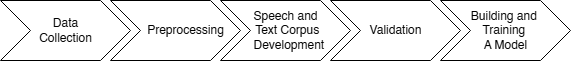
\includegraphics[width=\textwidth]{./figures/flowchart.png}
   \caption{Research Methodology}
	\label{fig:flowchart}
\end{figure}

\subsection{Data Collection}

\textbf{Collating Pre-existing Online Resources}

For the data collection, the researchers will make use of existing online resources from the website, Bible.com (see Appendix A for permission to use their resources). These resources include recordings and transcriptions of the Akeanon translations of the multiple books and chapters of the Bible.

\textbf{Compiling Akeanon Words}

The researchers will collect equivalent Akeanon words based off on the Swadesh 207 word-list and use the Aklanon to English Dictionary by \citeA{Reyes:1969} as reference. In addition to the Swadesh list, the researchers have reached out to Dr. David Zorc, one of the authors of the Aklanon-to-English Dictionary. Not only who he granted the researchers permission to use the dictionary, but he has also generously provided a soft copy of an existing database containing all the contents of the dictionary to the researchers. This database was shared courtesy of Dr. Jarrette Allen, a linguist who has also worked on the Akeanon language.

\textbf{Phonetic Transcription}

After compiling the Akeanon word lists, their phonetic transcription will also be encoded, using the work of \shortciteA{Rentillo:2022} as reference for Akeanon phonology. Audio transcriptions retrieved from the Bible.com will also have their phonetic transcriptions be encoded. For the phonetic transcription the researchers will seek assistance from Ms. Hazel Cipriano, a linguist who is also a native speaker of the language.

\textbf{Word Selection for Speech Corpus}

For building the speech corpus, the researchers will prioritize words from the Swadesh 207 list for the voice recordings. Additionally, to complete the selection of 1000 words that will be prepared for speakers to read, the researchers will collaborate with a linguistic expert during the selection.

\textbf{Voice Recording}

A total of 50 native speakers of standard Akeanon will be gathered for the recording of the generated word list. The researchers have also sought a collaboration with Aklan State University (ASU) - College of Teacher Education for the selection of speakers. The speakers will be of varying gender and age. Table~\ref{tab:native_speakers} shows the categories of native speakers. For the audio recording, the microphone that will be used will be Shure SM58 (dynamic, cardiod pick-up pattern) with a Focusrite Scarlett 2i2 audio interface, having Adobe Audition 2021 as the recording software. In case of unavailability, recording over a smartphone with noise-cancelling headphones would suffice. The audio file will be named in the following convention: \texttt{\textless gender\textgreater\_\textless age\_group\textgreater\_\textless speaker\_number\textgreater}.

\begin{table}[ht]
   \centering
   \caption{Categories of Native Speakers} \vspace{0.25em}
   \label{tab:native_speakers}
\begin{tabular}{|c|p{2in}|} \hline
   \centering Category & Subcategories \\ \hline
   Gender & Male \\
   & Female \\
   & Non-binary \\
   & Others \\ \hline
   Age Group & 12-15 \\
   & 16-30 \\
   & 31-45 \\
   & 46-65 \\ \hline
\end{tabular}
\end{table}

\subsection{Preprocessing}
For preprocessing audio files, Adobe Audition 2021 will be used for recording and audio processing, which will include normalization and noise reduction of the recorded audio. The cleaned up audio files will then be exported in a WAV format.

\subsection{Speech and Text Corpus Development}
The previous steps will set as a precedent for the speech and text corpus development. The development of the text corpus for the Akeanon language involves creating a comprehensive collection of audio transcriptions from pre-existing online resources, dictionary-based word list, and their respective phonetic transcriptions. For the speech corpus, the collated audio transcriptions and word list will be mapped with their corresponding voice recordings and will be annotated accordingly.

\subsection{Validation}
In collaboration with ASU College of Teacher Education and another linguistics expert, they will be aiding the researchers by validating the newly created text and speech corpora.

\subsection{Building and Training A Model}
To generate initial results for an ASR system, the researchers will build, train, and test a model using the Kaldi toolkit. Similar to the methods employed by \shortciteA{Panizales:2023}, a six-fold cross validation scheme will be used for testing and training the data. Finally, the researchers have decided to use a DNN model for training.

\section{Calendar of Activities}

% A Gantt chart showing the schedule of the activities should be included as a table. For example:

Table \ref{tab:timetableactivities} shows a Gantt chart of the activities.  Each bullet represents approximately
one week worth of activity.

%
%  the following commands will be used for filling up the bullets in the Gantt chart
%
\newcommand{\weekone}{\textbullet}
\newcommand{\weektwo}{\textbullet \textbullet}
\newcommand{\weekthree}{\textbullet \textbullet \textbullet}
\newcommand{\weekfour}{\textbullet \textbullet \textbullet \textbullet}

%
%  alternative to bullet is a star 
%
\begin{comment}
   \newcommand{\weekone}{$\star$}
   \newcommand{\weektwo}{$\star \star$}
   \newcommand{\weekthree}{$\star \star \star$}
   \newcommand{\weekfour}{$\star \star \star \star$ }
\end{comment}


\begin{table}[ht]   %t means place on top, replace with b if you want to place at the bottom
\centering
\caption{Timetable of Activities} \vspace{0.25em}
\makebox[\textwidth]{
\resizebox{1.2\textwidth}{!}{
\begin{tabular}{|p{2in}|c|c|c|c|c|c|c|c|c|} \hline
\centering Activities (A.Y. 2024-2025) 														& Sep & Oct  & Nov & Dec & Jan & Feb & Mar & Apr & May \\ \hline
Brainstorming and Selection of Topic      													& \weekone & \weektwo &  &  &  &  &  &  & \\ \hline
Drafting and Finalization of Chapter 1 - Introduction 										&  & \weektwo & \weekone &  &  &  &  &  & \\ \hline
Drafting and Finalization of Chapter 2 - Review of Related Literature      					&   &  & \weekthree &  &  &  &  &  &  \\ \hline
Preparation of Letters; UPVREB and Establish Communication for Collaboration     			&   & \weekone &  &  &  &  &  &  &  \\ \hline
Drafting and Finalization of Chapter 3 - Methodologies      								&   &  & \weekone & \weektwo &  &  &  &  &   \\ \hline
Proposal Document Creation in LaTex 														&   &  & \weekone & \weekone &  &  &  &  &  \\ \hline
Proposal Presentation 																		&   &  &  & \weekone &  &  &  &  & \\ \hline
Data Gathering 																				&   &  &  & \weekthree & \weekthree  &  &  &  & \\ \hline
Preprocessing 																				&   &  &  &  &  \weekone  & \weekthree &  &  &  \\ \hline
Drafting and Finalization of Chapter 4 - Results and Discussion 							&   &  &  &  &  & \weekone & \weektwo &  &  \\ \hline
Corpus Development and Validation															&   &  &  &  &  &  & \weekthree & \weekthree &  \\ \hline
Drafting and Finalization of Chapter 5 - Summary and Recommendation							&   &  &  &  &  &  &  & \weektwo & \weektwo \\ \hline
Drafting and Finalization of SP Defense														&   &  &  &  &  &  &  &  & \weekone \\ \hline
SP Defense																					&   &  &  &  &  &  &  &  & \weekone \\ \hline
\end{tabular}
}}
\label{tab:timetableactivities}
\end{table}

